\chapter{Anforderungen an die Energieverbundinsel}
	\label{Kap3}
	In diesem Kapitel wird das Konzept von dem Projekt Energieverbundinsel und die damit verbundenen Anforderungen mit Orientierung am SGAM entwickelt. Eine Erklärung zum Aufbau des SGAM wird in Anhang \ref{Kap:Anhang2} beschrieben. Die Abbildung \ref{Abb:SGAM_mapping_steps} zeigt das Vorgehen bei der Entwurfserstellung der Energieverbundinsel und Abbildung \ref{Abb:SGAM_map_overview} visualisiert das Ergebnis, des in diesem Kapitel erarbeiteten Modells. Bei einer Vertiefung des Ansatzes bieten sich Entwicklungstools für SGAM wie beispielsweise die SGAM Tool Box oder DISCERN an, welche aus Einarbeitungsgründen nicht verwendet werden. \\
	
	Nach der Bestimmung des Anwendungsfalles (Use Case), wird daraus die Funktions-Ebene  mit ihren zugehörigen Domänen und Zonen abgeleitet. Dies geschieht unabhängig von den einzelnen Akteuren, Kommunikationstechnologien, Daten- und Geschäftsmodellen. Diese werden im Folgenden anknüpfend an die Funktions-Ebene in den weiteren Interoperabilitäts-Ebenen (Component, Communication, Information and Business Layer) entwickelt. Die Energieverbundinsel kann als Nanogrid der einzelnen SGAM Domäne Customer Premises zugeordnet werden. \\ 
	
	Die Business-Ebene und die Zonen Enterprise und Market für eine kommerzielle Nutzung sind für die Simulation nicht erforderlich und werden nur skizziert. Auch die Kommunikations-Ebene und der ebenenübergreifende Aspekt Datenschutz, welcher vor allem bei Bezahlungsverfahren wichtig ist, werden nicht näher untersucht.\\
		
	\begin{figure}[h]
		\centering
		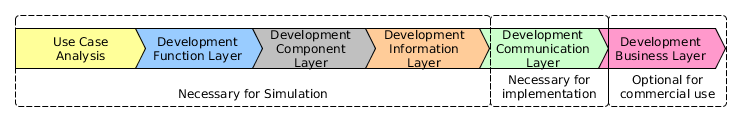
\includegraphics[width=14cm]{SGAM_mapping_steps}
		\caption{Prozess für Einordnung des Use Case im SGAM}
		\label{Abb:SGAM_mapping_steps}
	\end{figure} 
			
	Die meisten Bezahlsysteme der öffentlichen Ladesäulen konnten Ende 2017 mit öffentlichen Exploits gehackt werden, sodass beispielsweise Rechnungen zu Lasten voriger Ladepunktnutzer*innen und die Entwendung sensibler Daten nicht auszuschließen sind. \cite{CCC}  \cite{evsim}  \\ 	
	
	\section{Use Case Analysis}
		\label{Kap:Konzept_usecase}
			Der Anwendungsfall wird in Tabelle \ref{Tab:usecase} beschrieben und in Abbildung \ref{Abb:EMS} schematisch dargestellt. Die Abbildung fasst die Ladeinfrastruktur zu der CPS-unit \glqq Ladepunkte inkl. Laderegler\grqq zusammen und zeigt vereinfacht die Energie- und Datenflüsse. Zum Beispiel kommunizieren Ladepunktnutzer*innen mit dem EMS und dieses steuert die Energieflüsse. \\
            
            Das EMS kann sowohl in einer hierarchischen Struktur zentral gesteuert werden oder dezentral mit CPS-units, welche in einem Smart Grid miteinander kommunizieren und sich eigenintelligent selbst steuern. Eine dezentrale unhierarchische Kommunikationsstruktur ist deutlich komplizierter, daher wird für die Simulation der zentrale Ansatz gewählt. \\
            
		\begin{table}[h]
			\begin{tabularx}{\linewidth}{|c|X|}
				\hline 
				Name  		& Betrieb eines teilautarken Nanogrids mit Ladeinfrastruktur\\
				\hline 
				Aufgabenbereich 	& Überwachung und Regelung der Energieverteilung in\\
				(Scope) 			& teilautarkem Nanogrid mit konfigurierbarer Ladeinfrastruktur für E-Fahrzeuge durch zentrales EMS\\ 
				\hline 
				Ziel (Objective) 	& Überwachung und Regelung der Energieflüsse eines Nanogrids \\ 
				\hline
			\end{tabularx} 
			\caption{Name, Aufgabenbereich und Ziel des Anwendungsfall}
			\label{Tab:usecase}
		\end{table}
	
		\begin{figure}[h]
			\centering
			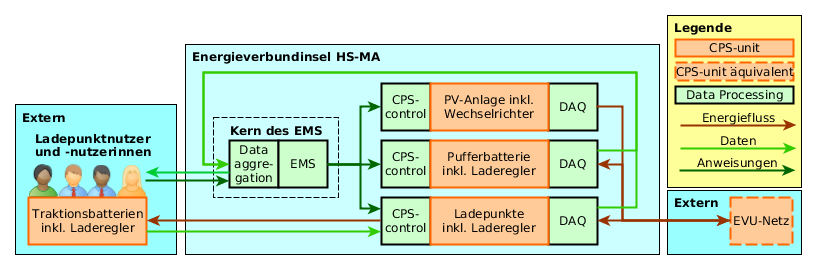
\includegraphics[width=14cm]{EMS}
			\caption{Schematische Darstellung der Energie- und Datenflüsse der Energieverbundinsel}
			\label{Abb:EMS}
		\end{figure}
			
		Anhand des Aufgabenbereichs wird eine Use Case Analysis durchgeführt. Alle Funktionalitäten und Akteur*innen  werden den SGAM-Zonen zugeordnet und in Abbildung \ref{Abb:usecaseanalysis} dargestellt. Eine Erklärung der Funktionalitäten ist in Tabelle \ref{Tab:usecase_zones} gelistet, die der Akteur*innen im Folgenden:\\
		
		\begin{itemize}
			\item Die CPS-units (EV, Ladepunktregler, PV-Anlage und Pufferbatterie) tauschen Energie im Nanogrid aus, werden überwacht und manche können gesteuert werden.
			\item Das Netz (Grid) tauscht mit dem Nanogrid Energie aus, kann jedoch nicht direkt gesteuert werden. 
			\item Benutzer*innen (User) konfigurieren den Ladevorgang, erhalten Daten und könnten optional Bezahlen.
			\item Das Bezahlungssystem (Payment System) für die Bestimmung der Nutzungskosten und Abwicklung der Zahlung ist optional.
			\item Das EMS (EMS) sammelt Daten, zeigt sie an, regelt die Energieflüsse durch Steuerung der CPS-units und macht die Energieflussregelung abhängig von User Konfigurationen
		\end{itemize}  

		\begin{figure}
			\centering
			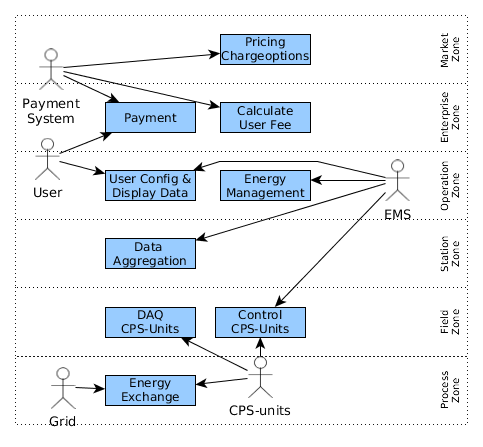
\includegraphics[width=0.6\textwidth]{usecaseanalysis}
			\caption{Usecase analysis der Energieverbundinsel mit teilautarker Ladeinfrastruktur}
			\label{Abb:usecaseanalysis}
		\end{figure} 
	

		\begin{table}
			\begin{tabularx}{\linewidth}{|c|X|}
				\hline 
				Zone & Beschreibung   \\ 
				\hline 
				Process 	& Austausch von Energie zwischen einzelnen CPS-units über Leitungen und Netzknoten \\ 
				\hline 
				Field 		& Messung und Steuerung übertragener Energie einzelner CPS-units \\
				\hline
				Station 	& Konzentration von Messdaten der einzelnen CPS-units \\
				\hline
				Operation 	& Konfiguration des Ladevorgangs und Regelung des Energymanagement aller CPS-units für den konfigurierten Ladevorgang \\
				\hline
				Enterprise 	& Kalkulation von Gebühren und Transaktionsverfahren für Bezahlungen \\
				\hline
				Market 		& Preisbilanzierung verschiedener Ladeoptionen \\
				\hline 
			\end{tabularx} 
			\caption{Beschreibung aller Funktionalitäten des Use Case mit Zuordnung der SGAM Zonen}
			\label{Tab:usecase_zones}
		\end{table}	
				
	\section{Funktionsebene des Konzeptes}
		\label{Kap:Konzept_func}
		Aus den bestimmten Funktionalitäten lassen sich die Funktionsebene ableiten und die funktionalen Abhängigkeiten bestimmen wie in Abbildung \ref{Abb:SGAM_map_func} gezeigt.\\
		
		Der Energieaustausch (Energy Exchange) von CPS-units wird gemessen (DAQ) und gesteuert (Control). Die aufgenommenen Messdaten einzelner CPS-units werden zentral gesammelt (Data Aggregation). Das Energiemanagement regelt Energieflüsse durch Steuerung der CPS-units und braucht dafür die konzentrierten Messdaten und User Konfigurationen (User Config).\\

		\begin{figure}[h]
			\centering
			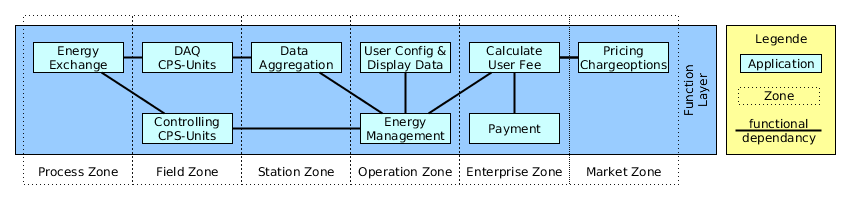
\includegraphics[width=14cm]{usecaseanalysis_func}
			\caption{Einordnung des Use Case in SGAM Zonen auf der Funktions-Ebene}
			\label{Abb:SGAM_map_func}
		\end{figure} 
	
		\subsection{Mögliche Konfiguration des Ladevorgangs} % Function Layer
			\label{Kap:Lademodelle}
			\subsubsection{Grundmodelle}
				In diesem Kapitel werden verschiedene Lademodelle für den Ablauf von Ladevorgängen für EV definiert. Diese können durch intelligente Regelung eines Energie- bzw. \ac{BMS} z.B. hinsichtlich minimaler Ladeverluste, Strompreisschwankungen, Netzstabilität oder \ac{SoH} optimiert werden. Dafür wurden einige Grundfunktionen in Tabelle \ref{Tab:Lademodelle} zusammengefasst und im Folgenden erklärt.\\
				
				\textbf{Kontinuierliche Ladung} ist eine Möglichkeit mit minimalen Ladeströmen, somit auch minimalen Ladestromverlusten, welche proportional zur Stromstärke im Quadrat auftreten. Kontinuierliche Ladungen führen zu einer gleichmäßig zeitlich verteilten, prognostizierbaren Last und beugen starken Leistungsgradienten vor.\\
			
				\textbf{Flexible Ladungen} müssen an bestimmte Vorgaben gekoppelt sein. Dieses Lademodell macht neben der vorraussichtlichen Anschlussdauer von weiteren Input-Parametern wie z.B. dynamischen Strompreisen oder Messwerten der Netzspannung bzw. -frequenz Gebrauch, welche in der Tabelle zusammengefasst als Ladekriterium benannt werden.\\ 
				
				\textbf{Sp"atladungen} können unter Umständen die Lebenszeit von Fahrzeugbatterien gegenüber einer kontinuierlichen Ladung erhöhen. LiFePO$_4$-Zellen, die z.B. oft in Notebookakkus oder E-Fahrzeugen verbaut werden, altern bei hohen Temperaturen und hohem SoC schneller. \cite[S.26]{FfE_Lademodelle_EAutos} Zu berücksichtigen ist dabei, dass Ladeströme sich ebenfalls auf den SoH auswirken. Vergleichsweise hohe Ströme werden durch höheren Verschleiß den SoH stärker beeinträchtigen, zu einer stärkeren Erwärmung und höheren Verlustleistungen führen.\\

				Je nach implementierter Hardware im Fahrzeug und verwendeter Ladesäulentechnik ist es theoretisch auch möglich zurück ins Netz zu speisen. Dieses Konzept wird \ac{V2G}, vom Fahrzeug ins Netz, genannt.\\
	
			\subsubsection{Beispiele kombinierter Modelle}
				Die Grundmodelle für Ladevorgänge lassen sich auch sequenziell zu komplexeren Lademodellen kombinieren. Im folgenden werden zwei einfache Beispiele mit Anwendungsfällen erläutert.\\
		
				\textbf{Kontinuierliche Ladung} und \textbf{Spätladung} lassen sich kombinieren zu einer später einsetzenden kontinuierlichen Ladung mit einer Ladeleistung zwischen der minimal für den Ladezeitraum nötigen und der maximal möglichen. Je genauer, die Auswirkungen auf den SoH der Batterie bestimmbar sind, desto genauer ließe sich der Ladealgorithmus einstellen, um den durch höhere Ladeströme bedingt größere Verschleiß zu berücksichtigen.\\
				
				\textbf{Sofortladung} und \textbf{flexible Ladung} lassen sich kombinieren. Im ersten Teil wird mit maximaler Leistung bis zu einem eingestellten SoC geladen und anschließend beginnt eine $flexible Ladung$ in welcher der vorher eingestellte SoC nicht unterschritten wird.  
		
				\begin{table}[h]
					\centering
					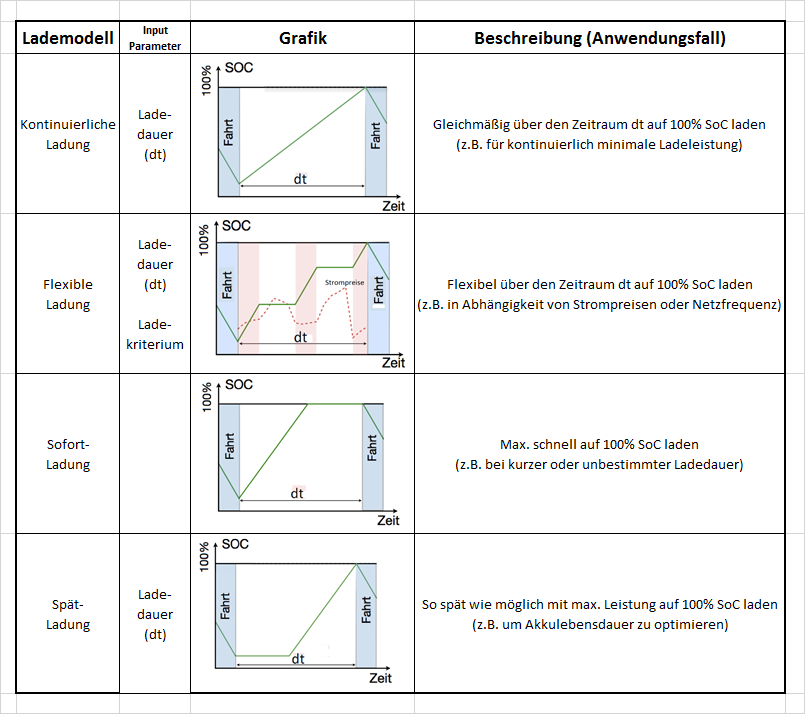
\includegraphics[width=16cm]{Lademodelle}
					\caption{Übersicht von Lademodellen nach \cite[modifizierte Grafiken]{FfE_Lademodelle_EAutos}}
					\label{Tab:Lademodelle}
				\end{table}

		\subsection{Konzept Energiemanagement}
		\label{Kap:DSM}
			Der Regelalgorithmus für das Energiemanagement eines EMS kann beliebig komplex gestaltet und hinsichtlich verschiedenster Aspekte optimiert werden. In diesem Kapitel wird ein einfacher Entwurf für die Laststeuerung \ac{DSM} mit einem Lademodus für die Pufferbatterie und drei konfigurierbaren Modi für die Ladepunkte gestaltet. \\

			Der logische Ablaufplan einer Simulation über T Zeitintervalle wird in Abbildung \ref{Abb:pap_dsm} gezeigt. Die For-Schleife entspricht einem Regelkreis mit der Regelgröße $P_{DSM}$, der Führungsgröße $0$ und der Stellgröße $P$, wobei in jeder Iteration die Planleistung von CPS-units der selben Priorität angepasst und damit $P_{DCM}$ abgeregelt wird.

			\begin{figure}[h] 
				\centering
				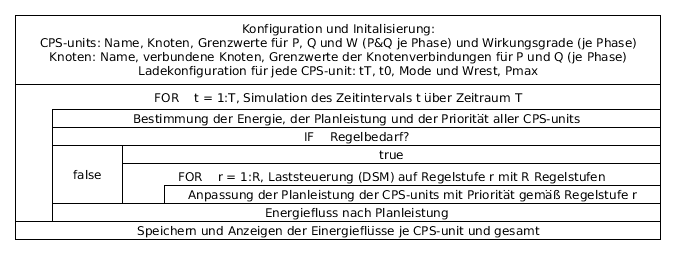
\includegraphics[width=\linewidth]{pap_dsm}
				\caption{Beispiel Ablaufplan für Energiemanagement mit mehreren Regelstufen}
				\label{Abb:pap_dsm}
			\end{figure}	
			
		\paragraph{Konfiguration} 
			% Ziel und Inputparameter
			User sollen die Lademodi $Mode$  Sofortladung (SofoL), Kontinuierliche Ladung (KontL) und Flexible Ladung (FlexL) einstellen und mit den Eingangsvariablen Anschlussdauer an Ladepunkt $dt$, zu ladende netto Batteriekapazität $W_{rest}$ und max. Ladeleistung $P_{max}$  konfigurieren können. \\  

		\paragraph{Bestimmung der Nennleistungen} %  P, Pn und \sum(Pn)	
			Die Planleistung $P_m$ einer CPS-unit $m$ wird zu Beginn eines Regelzyklus mit der zugehörigen Nennleistung $P_{m,n}$ gleichgesetzt $P_m = P_m,n~$. Diese wird abhgängig vom Lademodus bestimmt, bei Sofortladung (SofoL) mit der maximal möglichen Ladeleistung $P_{m,max}(SoC)$ und bei kontinuierlicher und flexibler Ladung (KontL und FlexL), so, dass der Energiebedarf $W_{m,rest}$ über den geplanten Anschlusszeitraum $dt_m$ durch eine kontinuierlich gehaltene Ladeleistung gedeckt wird. Die Nennleistung der Pufferbatterie $P_{m,n}(PB)$ entspricht der Summe aus der negativen PV-Ertragsleistung $P_{PV}$ und der Summe der Ladeleistungen von $M$ Ladepunkten. Alle Leistungswerte sind auf das Netz bezogen und entsprechen somit den Brutto-Ladeleistungen und Netto-Einspeiseleistungen. \\
			
			Für die Nennleistung innerhalb der Grenzwerte der verwendeten Ladepunkte gilt: \\
			$P_{m,n}(SofoL) = P_{m,max}(SoC)$  \\
            und ~ $P_{m,n}(KontL) = P_{m,n}(FlexL) = W_{m,rest}/dt_m$ \\
            und ~ $P_{m,n}(PB) = \sum_{m=1}^{M}(P_{m,n}) + P_{PV} $ 
			
			
			
		\paragraph{Bestimmung des Regelbedarfs}
			Ein Bedarf für die Regelleistung $P_{DSM}$ besteht, wenn die summierte Planleistung $P_{sum} = \sum_{m=1}^{M} P_m$ aller $M$ CPS-units mindestens in einer Phase an einem Knoten (Nanogrid) außerhalb der netzspezifischen Grenzwerte $P_{min,grid} ~\text{und}~ P_{max,grid}$ für die Übertragung zwischen Knoten der CPS-units und dem Netzknoten (Grid) liegt. Zu beachten ist, dass die PV-Anlage nicht am Netzknoten der Ladeinsel liegt und beim Energiemanagement nicht berücksichtigt wird. Im Verbraucherpfeilsystem gilt für $P_{DSM}$: 
					
		\begin{equation}
			\begin{split}
				P_{DSM} = P_{max}  - (P_{sum}) = P_{sum} > P_{max,grid} ~\text{bei geplanter Überlast}\\
				\text{und}~ P_{DSM} = 0 ~\text{für}~ P_{min,grid} < P_{sum} < P_{max,grid} ~\text{bei Betrieb in Normalbereich}\\	
				\text{oder}~ P_{DSM} =  P_{min}  - (P_{sum}) ~\text{für}~ P_{sum} < P_{min,grid} ~\text{bei geplanter Überversorgung}\\
			\end{split}  
		\end{equation}

		
			Im Nanogrid der Energieverbundinsel kann es aufgrund fehlender Energieerzeuger nur zu einem Regelbedarf an Erzeugungsleistung beziehungsweise Verbrauchsdrosselung kommen ($P_{sum}>P_{max,grid}$). Im Folgenden gilt daher pauschal $ P_{DSM} >= 0 $.
			

			
			
		\paragraph{Laststeuerung}
		% Allgemein
			Um den Regelbedarf $P_{DSM}$ an Regelleistung bereit zu stellen, können die Pufferbatterie mit $P_{max,PB}$ entladen und die genutzten $L$ Ladepunkte um die zugehörige Ladeleistungen $\sum P_{l} ~\text{mit}~ l=\big[1, ..., L\big]$ gedrosselt werden. Die neue Planleistung $P_{neu}$ kann mit einem Korrektursummanden $C$ oder einem Korrekturfaktor $k$ oder absolut mit $X$ beschrieben werden. \\ \\
			$P_{neu} = P + C \quad \text{mit} \quad P_{min} < P_{neu} < P_{max}$ \\   				
			
			In jeder Regelstufe teilen $L$ von $M$ CPS-units der zugehörigen Priorität den größtmöglichen Teil des neuen Regelbedarfs $P_{DSM,neu}$ unter sich auf. Dies geschieht gleichmäßig, bezogen auf die jeweils potientiell bereitstellbare Regelleistung. Für den Korrektursummand $C$ und -faktor $k$ gilt demnach: \\

			$P_{pot} = P - P_{min} \quad \text{für} \quad \sum_{1:l}^{L} P_{l,pot} > P_{DSM} >= 0$\\
            $\text{bzw.} \quad P_{pot} = P - P_{max} \quad \text{für} \quad P_{DSM} < 0 $ \\
			$C = P_{DSM} \frac{P_{pot}}{\sum_{1:l}^{L} P_{l,pot}}$ \\	
			
			Die Priorisierung von 1 bis 3 für CPS-units mit dem entsprechenden Lademodus wird in der folgenden Reihenfolge bestimmt: \\
			$ \text{prio} \big[1:3\big] \quad = \quad \big[\text{PB \quad FlexL \quad KontL oder SofoL}\big]$\\
							
			Der Algorithmus kann beliebig verändert und um Eingangsparametern erweitert werden wie z.b. mit $W$, $W_{max}$, $dt$ der Batterien (EVs und PB), PV-Leistung $P_{PV}$ und Wetter-/Lastprognosen.
			


% NOTE: HINWEISE ANFANG
% Hinweis: SoC Bestimmung		
	% Der anfängliche $SoC$ muss entweder durch die Kommunikation zwischen EV und Ladepunkt oder eine Usereingabe gegeben sein.\\ % NOTE: Ev. weg? Kommunikations-Ebene

% Hinweis Vorzeichensetzung
	% Das Verbraucherpfeilsystem wird auf alle CPS-units angewandt, sodass Leistungen mit positivem Vorzeichen einer Netzeinspeisung und negativem einem Netzbezug entsprechen. \\
% NOTE: HINWEISE ENDE
			
					
			
	\section{Informations- und Komponenten-Ebene des Konzeptes}
	\label{Kap:Konzept_comp}
		In Abbildung \ref{Abb:SGAM_map_all_total} wurde die SGAM-Visualisierung um die Informations- und Kom-\\ponenten-Ebene erweitert. Gezeigt wird die interebenen Kommunikation zwischen den Ebenen sowie die innerebenen, funktionalen Abhängigkeiten der User, Anwendungen, Info Objekten, Geräten und Netz. \\
		
		Die CPS-units (Ladepunkte, PB, PV-Anlage) tauschen Energie mit dem Netz aus und werden von Smart Metern überwacht und Controllern gesteuert. Die Messdaten werden von einem Data Collector gesammelt. Dieser kann mit dem EMS-Controller verbunden sein oder mit diesem in einem Gerät umgesetzt sein. Der EMS-Controller koordiniert mit den User Konfigurationen vom User Interface die CPS-Controller, um die Energie im Nanogrid zu managen. \\
		
		Im Folgenden werden die für die Berechnung der Energieflüsse verwendeten Datenmodelle beschrieben. Die Komponenten-Ebene wird nur skizziert, um den Prozess auf physikalischer Ebene besser zu veranschaulichen und für zukünftige Arbeiten eine Übersicht zu schaffen. Eine detaillierte Auflistung der Komponenten auf Prozess-Ebene wurde bereits erarbeitet. \cite{BA_Chris_Ong_2017}
	
%			\begin{figure}[h] % NOTE REF
%				\centering
%				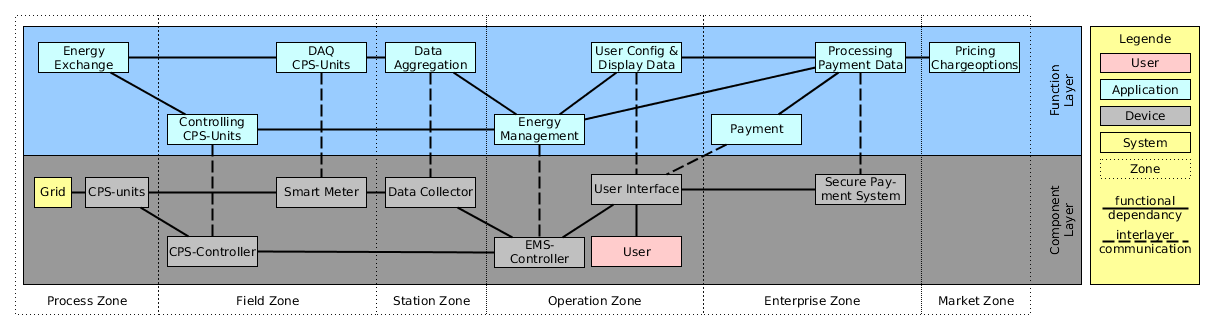
\includegraphics[width=14cm]{usecaseanalysis_func_comp}
%				\caption{Einordnung des Use Case in SGAM Ebenen Function und Component über alle Zonen}
%				\label{Abb:SGAM_map_func_comp}
%			\end{figure} 


			\begin{figure}[h] % NOTE REF
				\centering
				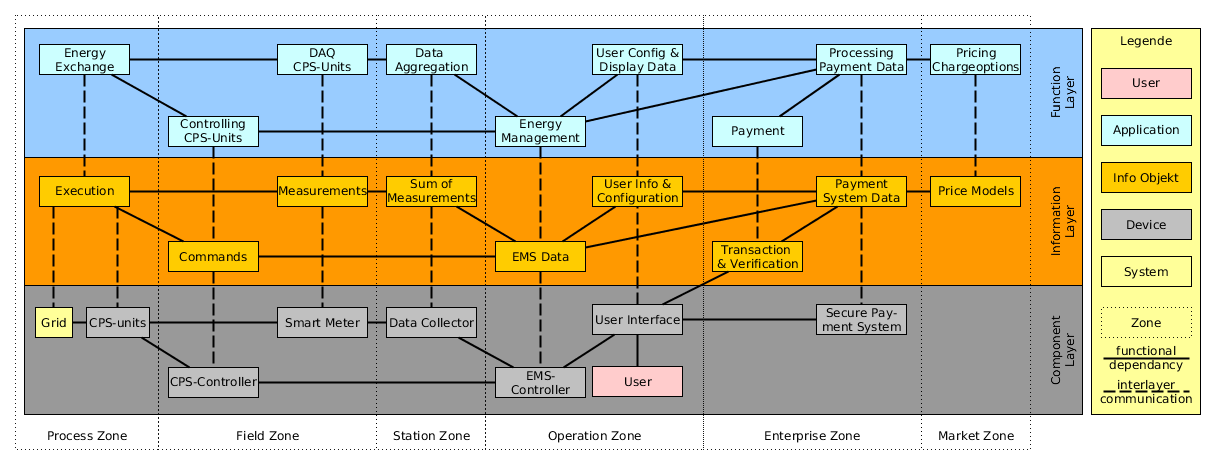
\includegraphics[width=14cm]{usecaseanalysis_all_total}
				\caption{Einordnung des Use Case in SGAM Ebenen Function, Information und Component über alle Zonen}
				\label{Abb:SGAM_map_all_total}
			\end{figure} 
					
		\subsection{Datenmodelle der Info-Objekte in Matlab Syntax}
			Um die in Kapitel \ref{Kap:Konzept_func} beschriebenen Funktionalitäten zu gewährleisten, werden die benötigten Informationen verschiedenen Info-Objekten zugeordnet. In diesem Kapitel werden hierfür die in der Simulation verwendeten Datenmodelle des Info-Objektes $EMS Data$ und $User Konfiguration$ erstellt. Für die $EMS Data$ wird die Datenstruktur für CPS-units (cps) und für Netzknoten (nodes) in Matlab Syntax definiert und ebenso die $User Konfiguration$ für Einstellungsparameter der Ladevorgänge (cpsuse) definiert. \\

			\paragraph{Prototyp Strukturdefinition der CPS-units (cps)}~ \\
			Die Attribute jeder CPS-unit werden, wie in Listing \ref{Code:prototype_cps} gezeigt, mit einem Array aus Zellen mit jeweils einer Varable des Datentyps $struct$ beschrieben. Jede Variable des Typs $struct$ ist wiederum ein Array mit Variablen (optional) unterschiedlicher Datentypen, die jeweils einem Feld (field) zugewiesen werden. Die Attribute einer $struct$ Variable können gelesen und beschrieben werden mit der Schreibweise <name struct variable>.<name struct field>, z.B. $cps.id~ = 'PV'$. Der Ansatz mithilfe von $struct$ Variablen bietet die Möglichkeit, im Nachhinein weitere Felder hinzuzufügen, ohne, dass die Funktionalität des bestehenden Codes beeinträchtigt wird. Denkbar sind beispielsweise die Temperatur, der SoH, oder dass bisher statische Eigenschaften wie der Wirkungsgrad dynamisch beschrieben werden. \\
            

            
	          \begin{lstlisting}[language=Matlab,caption=Funktion zur Strukturdefinition der CPS-units, label=Code:prototype_cps]
  % CPS STRUCTURE (consumer-producer-storage)
  % static fields
  cpsstruct.id   = '';            % string, name of CPS-units
  cpsstruct.node = '';            % string, name of connected node
  cpsstruct.pmin = [0,0,0];       % numeric (3x1), min. active power on phases [kW]
  cpsstruct.pmax = [0,0,0];       % numeric (3x1), max. active power on phases [kW]
  cpsstruct.qmin = [0,0,0];       % numeric (3x1), min. reactive power on phases [kvar]
  cpsstruct.qmax = [0,0,0];       % numeric (3x1), max. raective power on phases [kvar]
  cpsstruct.wmax = 0;             % numeric, netto battery capacity [kWh]
  cpsstruct.eta  = [0,0,0];       % numeric (3x1), power efficiencies eta(1), eta(2) 
  % and rate of energy degradation per hour eta(3) 
  % .w(t+1) = .eta(3)*.w(t) + .eta(1)*.p(t) with .p(t) > 0
  % .w(t+1) = .eta(3)*.w(t) + .eta(2)*.p(t) with .p(t) < 0 
  % efficiencies eta(1) for positive power, eta(2) for negative power
  % eta(3) as relative energydegradation per timeinterval
  
  % dynamic fields
  cpsstruct.prio = 0;           % scalar, priority
  cpsstruct.p = [0,0,0];        % numeric (3x1), sum of active power [kW]
                                % on each phase of every connected CPS-unit
  cpsstruct.q = [0,0,0];        % numeric (3x1), sum of reactive power [kW]
                                % on each phase of every connected CPS-unit
  cpsstruct.w = 0;              % scalar, netto capacity [kWh]
    	      \end{lstlisting}
			
			\paragraph{Prototyp Strukturdefinition der Ladevorgangskonfiguration der CPS-units (cpsuse) und der Netzknoten (node)} ~\\
             Für den Usecase der jeweiligen CPS-unit wie beispielsweise einstellbarer Ladesequenzen und für die Netzknoten (nodes) im Nanogrid wird jeweils der gleiche Ansatz mit Variable des Typs $struct$ gewählt. Der zugehörige Code wird in den Listings \ref{Code:prototype_cpsuse} und \ref{Code:prototype_node} gezeigt. \\
            

          \begin{lstlisting}[language=Matlab,caption=Funktion zur Strukturdefinition der CPS-Unit zugehörigen Usecases, label=Code:prototype_cpsuse]
  % CPSUSE STRUCTURE
  cpsusestruct.info = '';     % string, additional information
  cpsusestruct.id   = '';     % string, name of CPS-units
  cpsusestruct.mode = '';     % string, type of usecase e.g. 'KontL' for continuously charging
  cpsusestruct.w0   = 0;      % scalar, initial energy at start time t0
  cpsusestruct.wmax = 0;      % scalar, maximal energy (SoC 100 %)
  cpsusestruct.t0   = 0;      % scalar, start time, 
  cpsusestruct.tT   = 0;      % scalar, end time
          \end{lstlisting}			

          \begin{lstlisting}[language=Matlab,caption=Funktion zur Strukturdefinition der Netzknoten, label=Code:prototype_node]
  % NODE STRUCTURE
  % static fields
  nodestruct.id = {''};               % string, name of node
  nodestruct.link = {''};             % string array, name(s) of connected node(s)
  nodestruct.pmax = {[0,0,0]};        % numeric (3x1), max. sum of active power [kW]
                                      % on each phase of every connected CPS-unit
  nodestruct.qmax = {[0,0,0]};        % numeric (3x1), max. sum of raective power [kvar] 
                                      % on each phase of every connected CPS-unit

  % dynamic fields
  nodestruct.p = {[0,0,0]};           % numeric (3x1), sum of active power [kW]
                                      % on each phase of every connected CPS-unit
  nodestruct.q = {[0,0,0]};           % numeric (3x1), sum of reactive power [kW]
                                      % on each phase of every connected CPS-unit
          \end{lstlisting}
			
            \paragraph{Konfigurationsdaten in CSV-Format} ~\\
            Für eine einfache Initialisierung mit Wertzuweisungen der $struct$ Variablen, werden Matlab-Skripte in Form geschrieben, welche die entsprechenden Eigenschaften in tabellarischer Form aus CSV-Dateien auslesen und einem Array aus $struct$ Variablen zuweisen. Der Name der dritten CPS-unit wird beispielsweise aus dem Zellen-Array $cps$ mit $cps{3}.id$ abgerufen. Die CSV-Dateien mit Konfigurationsdaten sind in tabellarischer Form im Anhang in den Tabellen \ref{Tab:cfg_cps}, \ref{Tab:cfg_node}, \ref{Tab:cfg_cpsuse_wc}, \ref{Tab:cfg_cpsuse_nc} und \ref{Tab:cfg_cpsuse_bc} für alle drei Szenarien dargestellt. \\
			
%		\subsection{Process} % Component Layer	
%		\label{Kap:Process}
%		Ladeschränke:
%			https://www.lad-e.com/ladeschrank-f%C3%BCr-e-bikes/
%			https://rotstahl.de/produkt/akku-ladeschrank-e-bike-pedelec-cart/
%		
%			\subsubsection{Ladetechnik}
%			\label{Kap:Ladetechnik}
%				Die Ladetechnik der Pufferbatterie sollte die Möglichkeit bieten, die Batterie mit definierter Leistung über eine Stromregelung zu laden, wobei das Leistungslimit der Leistungselektronik im Laderegler die maximale Leistung der Batterie nicht übersteigen sollte. \\
%				
%				Für eine Netzintegration von Elektrofahrzeugen mit dem Ziel der Nutzung der Traktionsbatterien als Energiespeicher in einem Smart Grid (Vehicle to Grid, V2G), ist eine Ladetechnik notwendig, die bidirektionales Laden und damit Netzeinspeisungen ermöglicht.\\
%				
%				Einige E-Autos verfügen bereits über die Option einer Netzeinspeisung, darunter zum Beispiel 
%				der Opel Elektro-Meriva, 
%				der Nissan Leaf (CHAdeMO), e-NV200
%				der Mitsubishi EV (aka i-MiEV) ab Baujahr 4/2014 (CHAdeMO), 
%				der Mitsubishi Outlander Plug-In-Hybrid (PHEV)(CHAdeMO),
%				Theoretisch CCS-Anschluss, z.B. bei VW oder BMW\\
%				
%				
%			\subsubsection{Messtechnik}
%				Für die Leistungserfassung müssen für jede Phase Wirk- und Blindleistung gemessen werden. Für die Bestimmung des SoC der Traktions- und der Pufferbatterie ist die Messung der Batteriespannung, -ströme und -temperatur nötig. 
%				
%				Die Messtechnik muss für Spannungslevel in der Größenordnung von XYZ bis XYZ V und Ströme bis zu XYZ A ausgelegt werden. 
%			
%			\subsubsection{Steuertechnik}
%
%			
%			\subsection{Kommunikationstechnologie}
%			
%	
%						
%	\section{Softwareanforderungen} % Communication and Information Layer
%	\label{Kap:EMS_Anforderung_SW}
%
%		Zusammenfassung von CPS-units zu selbstregulierenden Microgrids	
%		Skalierbar für Anschluss zusätzlicher CPS-units/Microgrids		
%		Steuerung im Kleinen wie im Großen	
%		Idealerweise sowohl für Energiemanagement von realen als auch simulierten CPS-units
		

		
